% !TeX spellcheck = sk_SK-Slovak
\documentclass[a4paper]{article}
\usepackage[slovak]{babel}
\usepackage[utf8]{inputenc}
\usepackage[T1]{fontenc}
\usepackage{a4wide}
\usepackage{amsmath}
\usepackage{amsfonts}
\usepackage{amssymb}
\usepackage{mathrsfs}
\usepackage[small,bf]{caption}
\usepackage{subcaption}
\usepackage{xcolor}
\usepackage{graphicx}
\usepackage{enumerate}
\usepackage{hyperref}
\usepackage{fancyvrb}
\usepackage{listings}
%\usepackage{lstautogobble}
\usepackage{stmaryrd}

\lstset{basicstyle=\ttfamily,
	mathescape=true,
	escapeinside=||%,
	%autogobble
}


\fvset{tabsize=4}


\pagestyle{empty}
\setlength{\parindent}{0pt}

\newenvironment{modenumerate}
{\enumerate\setupmodenumerate}
{\endenumerate}

\newif\ifmoditem
\newcommand{\setupmodenumerate}{%
	\global\moditemfalse
	\let\origmakelabel\makelabel
	\def\moditem##1{\global\moditemtrue\def\mesymbol{##1}\item}%
	\def\makelabel##1{%
		\origmakelabel{##1\ifmoditem\rlap{\mesymbol}\fi\enspace}%
		\global\moditemfalse}%
}

\makeatletter
\def\@seccntformat#1{%
	\expandafter\ifx\csname c@#1\endcsname\c@section\else
	\csname the#1\endcsname\quad
	\fi}
\makeatother

\begin{document} 
	
\pagenumbering{arabic}
\pagestyle{plain}

\begin{center}
	\sc\large
	Programovanie paralélnych a distribuovaných systémov\\
	Domáca úloha 1 
\end{center}

Autor: Marián Kravec

\section{Časť 1}

Chceme dokázať, že program P3 
\begin{lstlisting}
Program P3
	initially r = 0
	assign r := max{ f(r), g(r), h(r) }
end{P3}
\end{lstlisting}

funguje, čiže spĺňa dve podmienky a to:

\begin{enumerate}
	\item Neurobí nič zlého – nepreskočí nejaký voľný spoločný termín“
	\item Urobí nakoniec niečo dobre – nájde spoločný termín
\end{enumerate}

Poďme to riešiť postupne:

\begin{enumerate}
	\item Chceme ukázať, že žiaden zo spoločných termínov (čiže ani najmenší) nebude preskočený. Dokážeme to sporom. Vznikajú dva možné prípady.
	\begin{itemize}
		\item $r$ túto hodnotu nadobudne ale neostane na nej, v takomto prípade vo chvíli keď túto hodnotu nadobudne bude podľa počiatočných podmienok platiť $f(r)=r$, $g(r)=r$, $h(r)=r$ a z toho vyplýva, že $max(f(r), g(r), h(r))=r$ čo v SPORE s predpokladom, že na tejto hodnote neostane
		\item $r$ túto hodnotu preskočí, keďže $r$ nikdy neklesá ak by táto situácia nastala muselo by existovať $r_1$(krok pred preskočením) a $r_2$(krok po preskočení) pričom pre preskočenú hodnotu spoločného termínu $r*$ platí $r_1 < r* < r_2$ a zároveň
		\\$max(f(r_1), g(r_1), h(r_1))=r_2$ avšak keďže predpokladáme, že naše funkcie vždy vrátia najbližší voľný termín (a $r*$ je voľný pre všetkých) takže $f(r_1) \leq r*$, $g(r_1) \leq r*$, $h(r_1) \leq r*$ z čoho vyplýva $max(f(r_1), g(r_1), h(r_1)) \leq r*$ z čoho vyplýva SPOR (keďže $r_2$ nemôže byť väčšie $r*$)
	\end{itemize}
	\item Potrebujeme ukázať, že tento kód nájde spoločný termín, keďže všetky funkcie kontrolujúce či je termín voľný vždy vráti hodnotu väčšiu nanajvýš rovnú vstupnej hodnote tak aj ich maximum nikdy neklesne, zároveň platí, že ak aspoň jednému termín nevyhovuje tak vráti väčšiu hodnotu z čoho vyplynie, že hodnota $r$ bude rásť kým nenastane hodnota vyhovujúca všetkým a keďže pracujeme s prirodzenými číslami a predpokladáme, že takáto hodnota existuje raz ju tento program dosiahne
\end{enumerate}

%\centerline{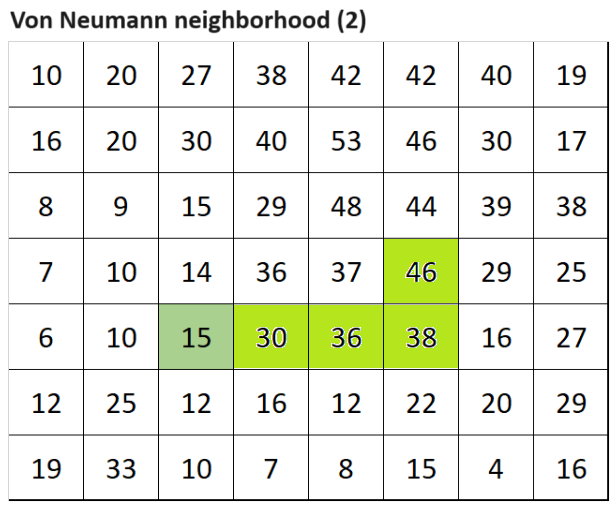
\includegraphics[width=0.6\textwidth]{von_2}} 
\newpage
\section{Časť 2}

Chceme dokázať, že program sort1 
\begin{lstlisting}
Program sort1
	assign
	$\langle \oblong$j: 0 $\leq$ j < N ::
		A[j], A[j + 1] := A[j + 1], A[j] if A[j] > A[j + 1]$\rangle$
end{sort1}
\end{lstlisting}
naozaj zoradí zoznam A.

Znovu chceme ukázať splnenie dvoch podmienok:
\begin{enumerate}
	\item V žiadnom kroku nebude zoznam menej utriedený ako v predchádzajúcom
	\item Od určitého bodu bude zoznam utriedený (a už sa nebude meniť)
\end{enumerate}

Poďme tieto podmienky dokázať:
\begin{enumerate}
	\item Uvažujme, že utriedenosť zoznamu budeme počítať ako počet dvojíc ktoré sú v nesprávnom poradí (väčšia hodnota má menší index) pričom platí, že zoradený zoznam má hodnotu 0. Tento program vymení hodnoty v prípade, že väčšia hodnota je pred menšou, čím odstráni jednu zle usporiadanú dvojicu čiže zníži počet zle usporiadaných dvojíc, z čoho vyplýva, že každým krokom je zoznam viac a viac utriedený
	\item Kým je zoznam neutriedený existuje aspoň jedna pozícia kde väčšie číslo je pred menším, keďže prehodenie každej dvojice je kontrolované nekonečne veľa krát, táto dvojica bude určite niekedy vymenená. Keďže takýmto prehodením sa počet možných takýchto dvojíc zníži (je ich nanajvýš toľko koľko je celkový počet neutriedených dvojíc o ktorých sme ukázali, že vymenením sa zníži) ale kým je zoznam neutriedený neexistuje, tieto výmeny sa budú diať kým už nebude 0 dvojíc v zlom poradí čiže je zoznam utriedený  
\end{enumerate}


\end{document}